% Adapted from ME310 document template
%%%%%%%%%%%%%%%%%%%%%%%%%%%%%%%%%%%

%%%%%%%%%BEGIN DOCUMENT STYLE SETTINGS%%%%%%%%%%%
% Don't modify this stuff unless you know what you're doing...
% We are using the "memoir" class, a widely used set of macros book-like documents.
% If you get errors that you are missing the "memoir" package you can download and 
% install it:   http://www.ctan.org/tex-archive/macros/latex/contrib/memoir/

% memoir document class for standard USA letter paper, printed one side
\documentclass[11pt,letterpaper,oneside]{memoir}
\chapterstyle{section}
\usepackage{graphicx}      			  % standard LaTeX graphics 
\usepackage{color}               	  % support for colored fonts
\usepackage{url}  \urlstyle{same}     % deal with url strings in bibliography
\usepackage{gensymb}
\usepackage{wrapfig}
\usepackage[font={small,it}]{caption}
\usepackage{dirtytalk}

%More special packages to help deal with long requirements tables 
%that might span multiple pages.
\usepackage{multirow} %deal with merged cells in tables
\usepackage{supertabular}
\usepackage{longtable}
\usepackage{morefloats}

\usepackage[pdftex,           %hyperlink cross references, etc.
    pdfsubject={ME112 Documentation},
    colorlinks={true},
    linkcolor={black},
    citecolor={blue},
    bookmarksopenlevel=1,
]{hyperref}				  

%The file "designreport.sty" should be in the same directory as this file.
% It contains formatting for page setup, titlepage, glossary, references, etc.
\usepackage{designreport}           
%%%%%%%END DOCUMENT STYLE SETTINGS%%%%%%%%%%

\setlength\parindent{0pt} % no indentation

%%%%%%%%%%BEGIN TITLE PAGE%%%%%%%%%%%%%%%%
%Replace the strings below with what's right  for you.

%%Insert your Document Title here. Use \\ to force a newline.
\title{Rockets IREC Systems Engineering Handbook}
\author{}
%% If you don't want it to use the printing date, replace "\today"
%% with the date that you want.
\date{\today}
%%%%%%%%%%%END TITLE PAGE%%%%%%%%%%%%%


%%%%%%%%%BEGIN ANY CUSTOM ABBREVIATIONS%%%%%%
% Define any useful abbreviations to save typing.
% For example:
\def\pmt{ {\em papier m\^{a}ch\`{e}} }  %Define "\pmt" to print "Papier Mache" with accents +1space
%%%%%%%%%END CUSTOM ABBREVIATIONS%%%%%%%%%


%%%%%%%%%%%%%%%%%%%%%%%%%%%%%%%%%%%%%%%%
%   BEGIN THE MAIN DOCUMENT
%%%%%%%%%%%%%%%%%%%%%%%%%%%%%%%%%%%%%%%%
\begin{document}

%If you want a figure on the cover page, this is where it goes.
%9 cm is about max figure height before messing up title spacing.
\begin{figure}[t]
\centering
  %An example cover image
  
\includegraphics[height= 9cm]{Figures/logo.png}
%\vspace{3 cm}    %Use this instead when you have no cover picture 
\end{figure}

%%%%%%%%%%%%%%%%%%%%%%%%%%%%%%%%%%%%%%
%Make the title page using arguments defined above.
\titlep

%%%%%%%%%%%%%%%%%%%%%%%%
% Load file "Executive.tex" for the Executive summary.
% Remember, this is a stand-alone section for executives to read.
%The executive summary is a special section that usually comes
% before the table of contents because it stands on its own.
\chapter{Executive Summary} 
\label{sec:executive}

The ultimate goal of the rockets team is to create and maintain a rocket engineering process that produces the outcomes we desire. Home-grown technology would follow best practices, create novel payloads and eventually get to space. This handbook provides a systems level overview of the rockets IREC process and is a step towards that goal.

%%%%%%%%%%%%%%%%%%%%%%%%
% TOC and LOF are automatically generated -- Note that sometimes have to "compile" Latex THREE
% times to update the main .aux files, the TOC etc. files, and finally the PDF output with all changes
% propagated to the printout.
% Make Table of Contents title smaller than a normal Chapter heading:
\renewcommand{\chaptitlefont}{\normalfont\Large\bfseries}
\newpage
\tableofcontents*  %asterisk to prevent it from getting a number
\renewcommand{\chaptitlefont}{\normalfont\Huge\bfseries}
%%%%%%%%%%%%%%%%%%%%%%%%

\chapter{Rocket Life Cycle}
\label{sec:rocketlifecycle}

This section is intended to give a high-level overview of the general process of engineering a rocket from scratch, regardless of the percentage of commercial off-the-shelf components used. The rocket life cycle begins once the team has committed to engineering a rocket for some purpose.

\section{Mission Planning}
\textbf{Evaluate goals}: SSI wide, rockets team wide, IREC team wide, subsystem. These should help form the guiding principles for what actually matters.\\

\textbf{Map out the external specifications for the rocket} (i.e. IREC rules and requirements). Keep those handy since it can be easy to forget about them after this phase of the life cycle. \\

\textbf{Identify key challenges} among all the requirements set on the team and the rocket. Try to use some team effort to begin to address mitigation strategies. This should be done throughout the process. \\

\textbf{Talk to other IREC teams} about past experiences. Identify teams you would like to emulate and stand on the shoulders of giants. In the past we've talked to: 
\begin{itemize}
\item Cal Poly
\item MIT
\item Oregon State University 
\end{itemize}
Here are some sample questions you can ask:
\begin{itemize}
\item What was your budget?
\item What did your timeline look like?
\item What was your biggest struggle?
\end{itemize}

\textbf{Optimize strategy for maximum points} within IREC. Look at the point spread and move on from there. Here is an excerpt of the 2016-17 IREC strategy:\\

\say{We also get 200 points for quality of design+build and amount of SRAD. The first big note we took from the category was that we cannot have tacked-on systems; everything needs to be planned out and well integrated. AKA if you think we are missing something, tell us ASAP so it doesn't become an afterthought. The second note is that a custom parachute is called out as being worth 25 points, so we will be attempting one (but not if it jeopardizes our altitude or recovery, which is worth far more.)}
\\

\textbf{Set safety factors}. This can be extremely difficult to do since there are often a lack of ways to do non-destructive tests. Here is a handy definition taken from our friends in Solar Car: \say{A factor of safety is a fudge factor that is actually a measurement of an engineer's confidence in their understanding of the design, manufacturing, and use case for an engineering project}.  \\

\textbf{Adhere to and set necessary loading conditions}. We have developed a set of loading conditions (but never enough). Similar to setting safety factors, this can be tough to accomplish without experience. They should look something like these:
\begin{itemize}
\item Recovery system is designed to separate at X m/s and all components must survive Y G's.
\item All components near charge must briefly survive Z temp.
\item All tubes and structural joints must withstand A mph wind shear occurring at a line across the middle of the rocket.
\end{itemize}
As Logan Herrera once said, \say{All loading conditions are supposed to actually match reality to B confidence level, and then we apply C safety factor}. \\

\textbf{Define subsystem}. Define purpose, upper bounds on size, and weight such that all goals, external specs, and strategy are satisfied. These definitions may be impossible to implement simultaneously; this is where the systems engineers work on compromise.  \\

\textbf{Project management begin}: set schedules, milestones, budgets, a communication plan, a task list, resource assessments and assignments, etc. This will be its own subsection, don't worry if this seems short.\\  

\textbf{Layout possible rocket configurations} based on your goals and IREC requirements. Pick one way of representing the rocket's length, weight, and space requirements and stick to it. For example, always have an updated Solidworks assembly which can spit out center of mass and locations of all components on the rocket worth modeling in simulation and integration. Have each subsystem 

\begin{figure}[h]
\centering
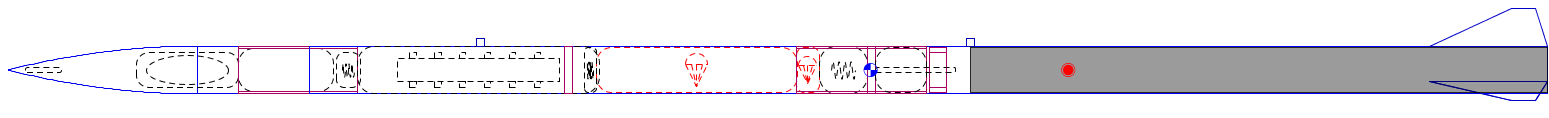
\includegraphics[width = 6in]{Figures/OR_layout.PNG}
\caption{OpenRocket layout}
\end{figure}

\textbf{Send configurations to simulations} for evaluation of feasibility and general order of magnitude (and a factor of 2 ;) analysis. \\

\textbf{Choose a rocket layout} after simulations come back. Add margin to both length and mass if you are aiming for an altitude-based goal. \\ 

\section{Prototyping}
This phase is pretty classic d.school. Begin work on concrete subsystem designs, exploring emph{different} ideas, so that we discover the best. We then choose our best guesses and present the rocket in a \textbf{Preliminary Design Review}. Throughout the process, each subsystem that can be non-destructively tested (or tested in pieces) is characterized as thoroughly as possible. 
\\

\section{Final Design Freeze}
% Design Development 
\chapter{Project Management}
\label{sec:project-mgmt}
   
% Design Development 
\chapter{Mission Planning}
\label{sec:mission-planning}
% Design Development 
\chapter{Simulations}
\label{sec:simulations}

% Design Development 
\chapter{Structures}
\label{sec:structures}

%The executive summary is a special section that usually comes
% before the table of contents because it stands on its own.
\chapter{Avionics} 
\label{sec:avionics}


%The executive summary is a special section that usually comes
% before the table of contents because it stands on its own.
\chapter{Recovery} 
\label{sec:recovery}


%The executive summary is a special section that usually comes
% before the table of contents because it stands on its own.
\chapter{Propulsion} 
\label{sec:propulsion}


%The executive summary is a special section that usually comes
% before the table of contents because it stands on its own.
\chapter{Integration} 
\label{sec:integration}


%The executive summary is a special section that usually comes
% before the table of contents because it stands on its own.
\chapter{On-site Engineering} 
\label{sec:on-site}


%% Appendices are below

%%%%%%%%%%%%%%%%%%%%%%%%%%%%%%%%
\include{Description}  %Description of the design and some explanation of its evolution

%%%%%BEGIN APPENDIX SECTIONS%%%%%%%%%%%%%%%
\begin{appendices}
 % Appendices are set up same as chapter sections
\chapter{Appendices}
       % There could be multiple appendix files like this
 \end{appendices}
 %%%%%END APPENDIX SECTIONS%%%%%%%%%%%%%%%
 
\end{document}

